% Chapter 4

\chapter{Implementation} % Main chapter title

\label{Chapter4} % For referencing the chapter elsewhere, use \ref{Chapter1} 

\lhead{Chapter 4. \emph{Implementation}} % This is for the header on each page - perhaps a shortened title

%----------------------------------------------------------------------------------------

% \emph{Diskuter de viktigste algoritmene og datastrukturene, og hvordan de utviklet seg, fremhev noen nye/originale funksjoner. Også diskuter hvordan du har tenkt å utføre testen din (validering og evaluering).}

This chapter will go through the algorithms and API calls being used by the application.

In addition to the three steps in chapter~\ref{Chapter3} -- ``data gathering'', ``sentiment analysis'', and ``rating prediction'' -- this chapter will also touch upon how the evaluation mechanisms were implemented. However, evaluation results and related discussions are deferred to chapter~\ref{Chapter5}.

\section{Languages and tools} % (fold)
\label{sec:languages_and_tools}

The system was implemented in the Python programming language, and has no further technical requirements. However, it supports using SQLite\footnote{\url{http://www.sqlite.org/}} to store and query various movie metadata, and to cache content classifications to avoid hitting the remote APIs too much during testing.

The final application is a highly configurable command-line tool. Its interface co-evolved with its requirements, and lets the user control most of its parameters. Figure~\ref{fig:tool_help} shows the result of running the final program with the \verb+--help+ argument.

\begin{figure}[h]
  \centering
    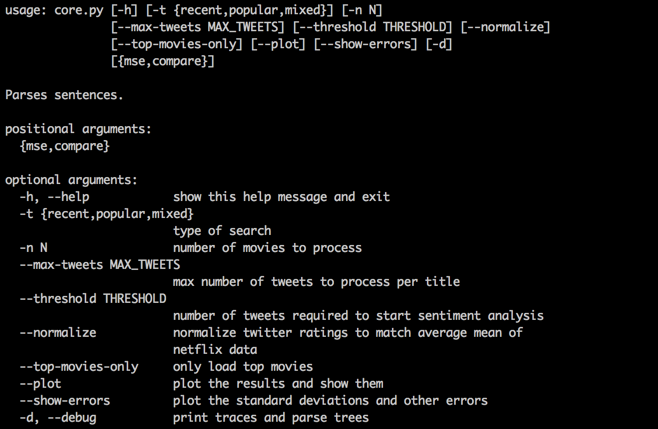
\includegraphics[width=.9\textwidth]{Figures/tool_help}
  \caption{Screenshot of the application's help menu.}
  \label{fig:tool_help}
\end{figure}

\subsection{Important data structures} % (fold)
\label{sub:data_structures}

The only somewhat complex entity being processed by the system is the Twitter messages. These are represented in the system as instances a simple \verb+Tweet+ class. It has a small set of default values and utility methods, but in practice, the objects behave as dictionaries.

Each \verb+Tweet+ object is augmented with additional metadata on its way through the system, until they are reduced to real-numbered predictions and discarded in the ``rating predicion'' execution step.

\section{Data gathering} % (fold)
\label{sec:data_gathering_impl}

As was soon found out after the initial tinkerings with the Twitter API began, the service has a high noise ratio. Therefore, every opportunity was taken to refine and tweak the search queries used to gather content. Luckily, the Twitter API has a quite extensive search interface, with many ways of tweaking the results (details in section~\ref{ssec:search_api}).

After much trial and failure, the following settings seem to yield good results for typical well-known movies:

\begin{description}
  \item[Title as exact phrase] \hfill \\
    Ensure that the title is searched for in its entirety, as a singular phrase and not just the individual words. In the Twitter API this is done by enclosing the title in quotation marks, as such: \verb+"pulp fiction"+, instead of \verb+pulp fiction+.
  \item[Exclude noisy terms] \hfill \\
  Exclude tweets containing the following terms\footnote{Any time a set of irrelevant results shared a common term, it would be added to the list. There are probably many ways of fine-tuning this further.}: ``download'', ``stream'', ``\#nw'', ``\#nowwatching'', and ``RT''.
\end{description}

Then remained the choice between the two modes of search: ``popular'', ``recent'', or the optional combination of the two.


% section data_retrieval (end)

\section{Sentiment analysis} % (fold)
\label{sec:sentiment_analysis_impl}

A central part of the system is the sentiment classification of the Twitter results. This sentiment analysis could well have been implemented locally, but for simplicity's sake it has been offloaded to an external service called DatumBox\footnote{\url{datumbox.com}}, as it seems to employ a reasonable choice of algorithm, and performs well enough for our needs.

This section will take an in-depth look at the techniques the DatumBox service utilizes.

% The sentiment classifier has three classes: ``positive'', ``negative'', and ``neutral''. The training set, consisting of 

To get us started, this is how DatumBox themselves describe their classifier~\cite{DatumBoxTwitterSentiment}:

\begin{quote}
  In order to detect the Sentiment of the tweets we used our Machine Learning framework to build a classifier capable of detecting Positive, Negative and Neutral tweets. Our training set consisted of 1.2 million tweets evenly distributed across the 3 categories. We tokenized the tweets by extracting their bigrams and by taking into account the URLs, the hash tags, the usernames and the emoticons.

  In order to select the best features we used several different algorithms and at the end we chose the Mutual Information. Finally after performing several tests with various models and configurations we selected the Binarized Naïve Bayes as the best performing classifier for the particular problem (strangely enough Naïve Bayes beat SVM, Max Entropy and other classifiers which are known to perform usually better than NB). To evaluate the results we used the 10-fold cross-validation method and our best performing classifier achieves an accuracy of 83.26\%.
\end{quote}

The next section will describe the naïve Bayes classifier in detail.

\subsection{The Naïve Bayes Classifier}
\label{ssec:nb_classifier}

The naïve Bayes classifier has several both strengths and weaknesses, and in many ways its weaknesses enable its strengths.

The most important of these qualities is found in the name of the classifier itself, ``naïve'', which comes from the algorithm's strong independence assumptions. These assumptions result in a very simple model that is both efficient to run and easy to implement. Although it tends to oversimplify the relations within the data, it often performs well enough to warrant the tradeoff.

The ``Bayes'' part of the classifier's name takes its name from the probabilistic model on which it is based, which strongly relies on Bayes' theorem.

The task of classifying text is viewed as a maximization problem, where we want to choose the maximally probable class based on our knowledge -- our evidence. The probability of class $C$ given $n$ features $F_1,...,F_n$ can be expressed in the following way:

\begin{equation}
  P(C|F_1,...,F_n)
\end{equation}

However, this model is infeasable if $n$ is very large, or each feature can take on a large number of values. Bayes' rule allows for the model to be reformulated in the following way:

\begin{equation}
  P(C|F_1,...,F_n) = \frac{P(C) P(F_1,...,F_n|C)}{P(F_1,...,F_n)}
  \label{eq:stat_dep}
\end{equation}

This is much more desirable, as calculating these factors is a much more tangible task than attempting to handle $P(C|F_1,...,F_n)$ directly.

As mentioned, the naïve Bayes has strong independence assumptions -- more specifically it assumes the features $F$ of the model to be conditionally independent, given the class $C$.

As an example, $A$ and $B$ are conditionally independent given $C$ if:

\begin{equation}
  P(A \cap B | C) = P(A|C) P(B|C)
\end{equation}

This allows us to rewrite~\eqref{eq:stat_dep} to the following:

\begin{align}
  P(C|F_1,...,F_n) &= \frac{P(C) P(F_1,...,F_n|C)}{P(F_1,...,F_n)} \\
                   &= \frac{P(C) \prod_{i=1}^n P(F_n|C)}{P(F_1,...,F_n)}
\end{align}

However, the $P(F_1,...,F_n)$ in the denominator is constant. For the classifier we only need the probabilities relative to each other, and this lets us simplify a bit further:

\begin{equation}
  P(C|F_1,...,F_n) \propto P(C) \prod_{i=1}^n P(F_n|C)
  \label{eq:bayes_final}
\end{equation}

By maximizing~\eqref{eq:bayes_final} using the maximum a posteriori decision rule (MAP), we can build our classifier.

\begin{equation}
  \text{classify}(f_1, ..., f_n) = \argmax_c P(C = c) \prod_{i=1}^n P(F_i = f_i| C = c)
\end{equation}

\subsection{Other issues}

When calling the DatumBox API, the best results were achieved when removing the movie title itself from the query. Quite a lot of titles have sentiment-carrying words in their titles\footnote{``Breaking Bad'' consequently scoring way below ``Cheers'' was a rather clear cut case.}, and this obviously confused the classifier quite a bit.

% section sentiment_analysis (end)

\section{Evaluating sentiment} % (fold)
\label{sec:evaluating_sentiment}



% section evaluating_sentiment (end)
